\chapter{Suites et séries de fonctions} % (fold)
\label{chap:Suites et séries de fonctions}

\section{Position des problèmes} % (fold)
\label{sec:Position des problèmes}

\begin{Definition}[colbacktitle=red!75!black]{Suite de fonctions, Séries de fonctions}{}

  Soit $X$ une partie de $I$. 
  \begin{itemize}

      \item Une \textbf{suite de fonctions} sur $X$ est la donnée de 
        \begin{equation}
          (f_n) _{n \in \mathbb{N}} \text{ où } f_n \in \mathscr{F}(X, \mathbb{K})
        \end{equation}

      \item Soit $(f_n) _{n \in \mathbb{N}}$ est une suite de fonction, la série de cette suite de fonction est $\sum_{}^{}f_n$.
  \end{itemize}
\end{Definition}

\begin{tcolorbox}
    Questions : 
    \begin{itemize}

        \item Qu'est-ce que le sens de la \underline{convergence} pour une suite de fonctions ? 

        \item Qu'en est-il de régularité ? Les fonctions peuvent être continues mais la limite n'est pas.

    \end{itemize}
\end{tcolorbox}

% section Position des problèmes (end)

\begin{Example}{}{}
  Considérons la fonction avec $x \in [0, \frac{\pi}{2}]$, 
  \begin{equation}
    f_n = \sin(x) ^{n}  \underset{n \to +\infty}{\longrightarrow} f = \begin{cases}
      0 \text{ si } x \in [0, \frac{\pi}{2} ]\\ 1 \text{ si } x = \frac{\pi}{2} 
    \end{cases}
  \end{equation}
\begin{center}
    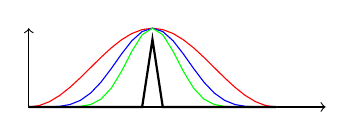
\begin{tikzpicture}
      \draw [<->] (0,1)--(0,0)--(1.2*pi,0);
      \draw[red,domain =0:pi] plot (\x ,{(sin(\x r)) ^2});
      \draw[blue,domain =0:pi] plot (\x ,{(sin(\x r)) ^5}); 
      \draw[green,domain =0:pi] plot (\x ,{(sin(\x r)) ^10}); 
      \draw[thick,domain =0:pi] plot (\x ,{(sin(\x r)) ^10000}); 
    \end{tikzpicture}
\end{center}
\end{Example}


\newpage

\section{Types de convergences} % (fold)

% section  (end)
\subsection{Convergence simple} % (fold)

\begin{Definition}[colbacktitle=red!75!black]{Convergence Simple}{}

  Pour $(f_n ) _{n \in \mathbb{N}} \in \{ \mathscr{F}(\Omega, F)\} ^{\mathbb{N}}$ avec $(F, \| . \|_F)$ un espace vectoriel normé, $f_n$ \textbf{converge simplement} vers $f \in \mathscr{F}(\Omega,F)$ si : 
  \begin{equation}
   f_n  \overset{CVS}{\underset{n \to +\infty}{\longrightarrow}} f  \iff \forall \omega \in \Omega, \; f_n(\omega)  \overset{\| . \|_F}{\underset{n \to +\infty}{\longrightarrow}} f(\omega)
  \end{equation}
\end{Definition}

Remarques : 

\begin{itemize}

    \item $F$ pourrait être un espace métrique $(E,d)$ : 
      \begin{equation}
        d(f_n(\omega), f(\omega))  \underset{n \to +\infty}{\longrightarrow} 0
      \end{equation}

    \item Quand il y a une norme sur l'ensemble des fonctions : Soit $f_n \in \mathscr{C}([a,b], \mathbb{R})$,

  \begin{equation}
    \forall \omega \in \Omega, \; f_n(\omega)  \overset{\| . \|_ {\infty, [a,b]}}{\underset{n \to +\infty}{\longrightarrow}} f(\omega) \iff \| f_n - f \| _{ \infty, [a,b]}  = \underset{x \in [a,b]}{\sup} |f(x)|\underset{n \to +\infty}{\longrightarrow} 0
  \end{equation}

   \item Quand il y a une semi-norme (norme mais sans la propriété de la caractère défini : $\forall x \in E$, $N(x) =0 \implies x = 0_E$) sur l'ensemble des fonction. 

     \begin{tcolorbox}
       Exemple de semi-norme : $\mathcal{L} ^{2}(\Omega, \mathbb{R}) = \{f : \Omega \to \mathbb{R}, \; f ^{2} \text{ intégrable sur } \Omega\}$ dans $(\Omega, \mathscr{T}, \mu)$ un espace mesuré : 
         \begin{itemize}

             \item C'est un espace vectoriel
              \item On peut construire un semi-norme : 
                \begin{equation}
                  f \underset{\| . \|_{2, \Omega}}{\mapsto} \sqrt{\int_{
                      \Omega
                  }^{} f ^{2} \mathrm{d}\mu}
                \end{equation}

                car $\{ \| f \| _{2,\Omega} = 0\} = \{f : \Omega \to \mathbb{R}, \; f = 0 \text{ p.p.}\}$

         \end{itemize}
     \end{tcolorbox}

   \item Quand on a une (presque)-norme : $\underline{N} :E \to [0, +\infty]$ avec $0 \times \infty = 0$ : 
     \begin{equation}
       f_n  \underset{n \to +\infty}{\longrightarrow}  f \iff \underline{N}(f_n-f)  \underset{n \to + \infty}{\longrightarrow} 0
     \end{equation}

     \begin{tcolorbox}
       Exemple de (presque)-norme : $\| f \| _{\infty, \mathbb{R}} = \underset{x \in \mathbb{R}}{\sup} |f(x)| \in [0, {\color{red} + \infty]}$ : 
       \begin{equation}
         f_n : x \mapsto x + \frac{1}{n}  \underset{n \to + \infty}{\longrightarrow}  \mathrm{id}_ \mathbb{R}
       \end{equation}
     \end{tcolorbox}

\end{itemize}



% section Convergence simple (end)

\subsection{Convergence uniforme} % (fold)
\label{sub:Convergence uniforme}

\begin{Definition}[colbacktitle=red!75!black]{Convergence uniforme}{}
Soit $(f_n) _{n \in \mathbb{N}} \in \{ \mathscr{F}(\Omega, E) ^{\mathbb{N}}$ où $E$ un espace métrique (de même pour les autres), la suite \textbf{converge uniformément} sur $\Omega$ vers $f$ si : (lorsque $E$ un espace vectoriel normé, on notera une (presque)-norme)
\begin{equation}
  f_n  \overset{CVU}{\underset{n \to +\infty}{\longrightarrow}} f \iff \underset{x \in \Omega}{\sup} \; d (f_n(x), f(x))  \underset{n \to + \infty}{\longrightarrow}  0 \text{ ou } \| f_n-f \| _{\infty, \Omega} \overset{Not}{=} \underset{x \in \Omega}{\sup}\; \| f_n(x)- f(x) \|_F  \underset{n \to +\infty}{\longrightarrow} 0
\end{equation}
\end{Definition}

Remarque : 
\begin{itemize}

    \item Uniforme en mathématiques signifie indépendant d'un paramètre. L'écriture de convergence simple : 
      \begin{equation}
        \forall x\in A, \; \forall \varepsilon >0, \; \exists N \in \mathbb{N}, [n \ge N] \implies [d(f_n(x), f(x)) \le \varepsilon]
      \end{equation}
      avec $N = N(x, \varepsilon)$ Mais l'écriture de convergence simple : 
      \begin{equation}
        \forall \varepsilon >0, \exists N \in \mathbb{N}, [n \ge N] \implies [{\color{red} \forall x\in A}, d(f_n(x), f(x)) \le \varepsilon]
      \end{equation}
      avec $N = N(\varepsilon)$
\end{itemize}

% subsection Convergence uniforme (end)

\begin{Prop}{De CVU vers CVS}{}
Soit $(f_n) _{n \in \mathbb{N}} \in \mathscr{F}(\Omega, E) ^{\mathbb{N}}$, alors 
\begin{equation}
  [f_n  \overset{CVU}{\underset{n \to +\infty}{\longrightarrow}} f] \implies
  [f_n  \overset{CVS}{\underset{n \to +\infty}{\longrightarrow}} f]
\end{equation}
\end{Prop}

\begin{myproof}{}{}
  [$\exists b\in B,\; \forall a \in A,\; \mathscr{P}(a,b)$] donc [$\forall a\in A, \; \exists b\in B,\; \mathscr{P}(a,b)$], réciproque fausse car lorsque $\underset{x \in \Omega}{\sup} N(x, \varepsilon)=+\infty$, $N(\varepsilon)$ n'existe plus.
\end{myproof}





% chapter Suites et séries de fonctions (end)
